\chapter{Implementation}


\section{Hierarchy of Arrays}

The API of an array is defined by an interface called INDArray which has a dense implementation for each backend: NDArray class for the CPU and JCublasNDArray class for the GPU. But since most of the operations and methods are shared between the two backends, they are implemented in an abstract class called BaseNDArray.

Adding sparse representations asked two questions:
\begin{enumerate}
 	\item What can be shared with the dense arrays ?
	\item What can be between the different sparse arrays and what are format-specific ?
\end{enumerate}

To answer those questions, we need to go a little bit deeper in the implementation. 

The dense implementation includes methods that are inherently related to the way dense ndarray is internally made, and other methods are related to the generic parameters such as the shape or are utility method.

The first type of methods is not useful in case of sparse. Dense and sparse ndarrays aren't built in the same manner. Methods such as \textit{getStrides} aren't relevant in the sparse context. Reciprocally the sparse array will need methods which will be irrelevant in the dense context.

We encounter the same situation between the different sparse formats. Some will need utily methods that the other ones won't need.

But everything has to be defined in the INDArray interface. To avoid code duplication, everything than can be shared should be implemented in the higher level of the hierarchy. The methods that are not compatible with a type of ndarray will simply throw an unsupported operation exception.

The drawback brought with this solution is that we always need to verify the type of the ndarray before doing any operations.

// TODO update schema
 
\begin{figure}[H]
	\begin{center}
		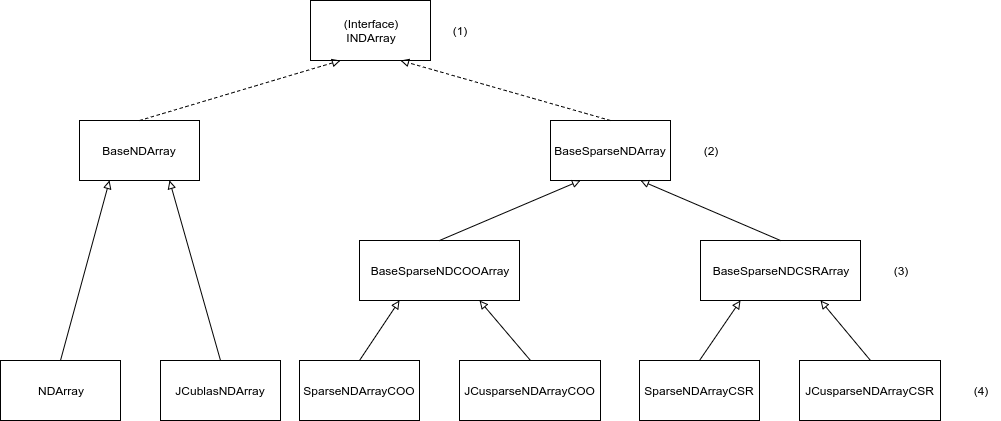
\includegraphics[width=6.5in]{images/INDArrayHierarchy.png} 
		\label{fig:hierarchy}
		\caption{Arrays hierarchy in Nd4j}
	\end{center}
\end{figure}


\section{Limitations and Constraints}

Nd4j has been made in the perspective of dense arrays. The design has been thought and optimized regarding the dense implementation which brings some constraints to implement the sparse representation
\subsection{storing off-heap}

// TO ASK TO RAVER:
What are the advantages for storing data off-heap ? Why Garbadge collector is a bad thing ?

What the idea behind the workspaces and how does it work ?

Before the workspaces, data were already stored off-heap. What do workspaces bring new ? How could 

Why it wasn't possible to have arrays of databuffers native side ? what we had to flatten everything?


\subsection{Workspaces}
\subsection{DataBuffers have a fixed length}

explain what is in the ToC doc

--------
-> we can reallocate memory from java side but it's impossible from native side. so we need to overallocated to the max result size before any operations !

1 - estimate the size needed (only the size of the view -> which avoid to allocated at the max size of the array - it wouldn't fit in memory)
2 - reallocate
3 - perform the op

-> add in op interface


\section{CSR Matrices}
\subsection{Structure}

The representation uses 4 data buffers to encore a CSR matrix. One for the non-zero values, one for the columns indexes and two for the row pointers (to the beginning and to the end of each row).

\subsection{Put a value}

To insert a new value or to update an existing non-null value, we need to identify where the values of row we want ot insert to are located in the values buffer and in the columns buffer. The beginning and end of rows pointers give us the range of indexes.

While iterating over the range of values, if we find a value with the same column index than the one we want to insert to, we can update the values and nothing needs to be changed in the three other buffer. 

However if there is no value with that column, we need to insert a new one at the correct position. Then we need to update the end of row pointer for this row. Finally each row pointers that come after need to be increment by one.


-- ADD pseudo code for putscalar of csr




\subsection{Get a Sub-array}

\begin{enumerate}
\item First, we need to resolve the index to get the new shape of the array, the new rank, etc. In the case we use the resolution of the dense array but we are only interested in
\begin{itemize}
	\item the shape: an array with two elements containing the new shape of the sub-array.
	\item the offsets: an arays with two elements that indicate the first row and the first column that belongs to the sub-array.
	\item the offset: indicates the position in the databuffer of the first element that belongs to the sub-array.
\end{itemize}
 \item Sometimes the offsets are equals to zeros while having a non-null offset. In this case we need to override the offsets.
\begin{lstlisting}
	 offsets[0] = (int) resolution.getOffset() / shape()[1];
	 offsets[1] = (int) resolution.getOffset() % shape()[1];
\end{lstlisting}
\item With the offsets we can now compute the first and the last position of each dimension.
\begin{lstlisting}
	long firstRow = offsets[0];
	long lastRow = firstRow + shape[0];
	long firstColumn = offsets[1];
	long lastColumn = firstElement + shape[1];
\end{lstlisting}
\item Now we have the bounds for each dimension, we can reconstruct the new beginning and end of row pointers et the columns indexes.
\end{enumerate}

% put the code in annex?

\subsection{Limits with this format}

This formats only works with two dimensions and cannot be extended to tensors. Therefor it makes it difficult to be compatible with the API.
Moreover the operations to get or put values aren't straightforward. Several step are necessary before accessing the value.

\section{COO Tensors}
\subsection{Naive implementation}

Based on the description in \ref{sssec:coo} the COO encoding needs one databuffer to store all the non-null values and one for the indexes of each values. 

An easy solution would have been to store the indexes into a multi-dimension array of databuffers: One databuffer for each value, or one databuffer for each dimension. Due to the native constraints that makes hardly manageable to have such arrays (Difficulty to pass the array to the native side and cuda side), we choose to flatten the indexes into one databuffer.

\begin{figure}[!h]
	\subfloat[each index is stored contiguously]{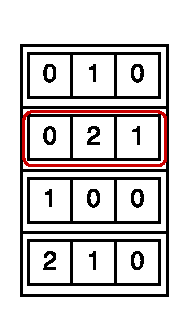
\includegraphics[width=1.5in]{images/indexesCoo_a.pdf} \label{fig:cooIdxA}}
	\subfloat[Each dimension is stored contiguously]{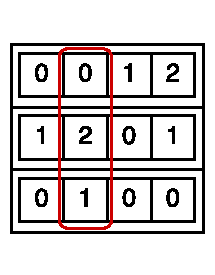
\includegraphics[width=1.5in]{images/indexesCoo_b.pdf} \label{fig:cooIdxB}}
	\subfloat[Indexes are flatten]{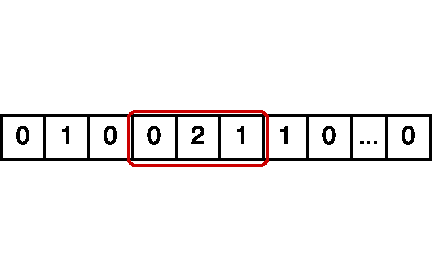
\includegraphics[width=2.5in]{images/indexesCoo_c.pdf} \label{fig:cooIdxC}}
	\hfill
	\caption{Illustration of the different possible datastructure for storing the indexes  [0, 2, 1] of a value $v$ }
\end{figure}

% TODO regenerate the schema - too much bottom margin

But this implementation makes difficult to be compliant with the API. It brings several issues:
\begin{itemize}
	\item The key of views is the sharing of their data. In case of COO format, views have to share the data buffer and the indexes buffer. Without the indexes it is not possible to add a value in the original array by adding it in a view. If we only put the new value in the shared value buffer without updating the indexes, the original array would have a value buffer bigger than its indexes buffer and there would be an offset between the values and the indexes. 
	
	Even when sharing both buffers, how would we know which value is included in the view and which is ot? 	
	
	\item The coordinates of a value in a view are not necessary the sames of the same value in the original array. 
		
	They can be offset if dimension is partially included in the view. Figure \ref{fig:viewOffset} shows a matrix an a view (in red). The value$ v_{i}=5$ would have the coordinates [1, 1] in the original array while it has the coordinates [0, 0] in the view. How the indexes can be translated between views?
	\begin{figure}[!h]
		\centering
		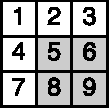
\includegraphics[width=0.8in]{images/viewIndexOffset.pdf}
		\caption{A $3\times 3$ matrix with a $2\times 2$ view in red}
		\label{fig:viewOffset}
	\end{figure}

	\item kmk
\end{itemize}

\subsection{More parameters are needed to define the tensors}


\subsubsection{All and Interval Indexes}
\subsubsection{Point Index}
\subsubsection{Specified Index}
\subsubsection{New Axis Index}

\subsection{Computations of the the Parameters}
\subsubsection{Computation of the Sparse Offsets}
\subsubsection{Computation of the Flags}
\subsubsection{Computation of the Hidden Dimensions}

\subsection{Sparse Indexes Translation}
..